%!TEX root=../oi-magistr-si.tex
\section[WA2 - Java EE]{Architektura Java EE, funkce jednotlivých vrstev, životní cyklus standardizovaných komponent Java EE, návrhové vzory využitelné v architektuře webové aplikace.}

Distribuce Javy se liší podle jejího zamýšleného použití:
\begin{itemize}[itemsep=0px]
\item \textbf{Java ME} (\textit{Java Micro Edition}) pro mobilní aplikace, omezený rozsah funkcí.
\item \textbf{Java SE} (\textit{Java Standard Edition}) pro desktopové aplikace.
\item \textbf{Java EE} (\textit{Java Enterprise Edition - J2EE}) pro webové aplikace.
\end{itemize}

\subsection{JAVA EE}
\begin{itemize}[itemsep=0px]
\item Komponentový přístup.
\item Komponenty mohou být distribuované na různých strojích (klient, server, DB).
\item Aplikace rozdělena do vrstev.
\item serverová část aplikace bývá nasazena na aplikačním serveru, který umožňuje zpracování více požadavků naráz (multi-threading). Nasazení znamená zabalení celého projektu do např. WAR archivu, který obsahuje vše potřebné (zdrojové třídy, statické resources, použité knihovny).
\item Podpora JNDI, java beans, JAAS (autentizace), JMS (Java Messaging Service), servlety, transakce (JTA – Java Transactions API).
\end{itemize}

\begin{figure}[h!]
\centering
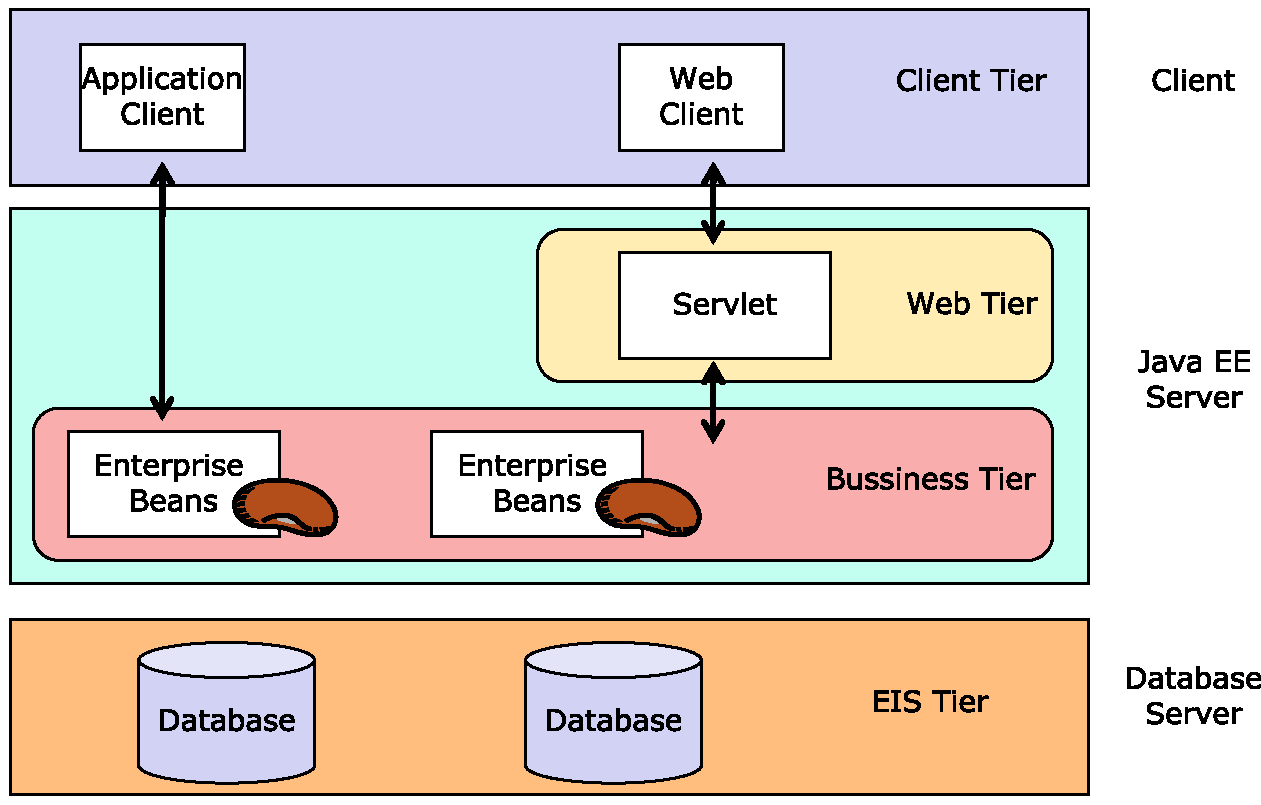
\includegraphics[width=140mm]{16/images/java-ee-arch}
\end{figure}

\paragraph{MVC} Většinou je aplikace navržena podle vzoru MVC. Jedná se o konkrétní aplikaci vzoru oddělení zodpovědností (\textit{separation of concerns}), který předepisuje vysokou kohezi jednotlivých komponent. Každá komponenta by měla mít vysoce soudržnou sadu zodpovědností a všechny ostatní požadavky by měla delegovat komponentám, které jsou úzce specializované zase na jinou činnost.

MVC tedy odděluje zodpovědnosti za data (model), pohled na data (view) a manipulaci s pohledem na data (controller). Aplikace je rozdělena na tři vrstvy: datovou, prezentační a ovladače (controllers). Tyto tři vrstvy jsou na sobě nezávislé a umožňují snadné vyjmutí jedné vrstvy a nahrazení jinou implementací.

\subsection{Servlet}
\textbf{Servlet je třída}, která rozšiřuje schopnost webserveru. \textbf{Zpracovává} a odpovídá na \textbf{požadavky} z webových klientů, typicky HTTP requestů. Třída musí implementovat rozhraní \texttt{javax.servlet.Servlet}, které definuje metody životního cyklu vyžadované servletovým kontejnerem. Při použití na webu servlet typicky rozšiřuje třídu \texttt{javax.servlet.http.HTTPServlet}, která definuje metody na zpracování jednotlivých HTTP požadavků: \texttt{doGet()}, \texttt{doPost()}, atd.

\begin{verbatim}
public class MujServlet extends HttpServlet { 
    @Override
    public void doGet(HttpServletRequest req, HttpServletResponse res) {
        res.getWriter().write("<html>Text ve formatu HTML</html>");
    }
}
\end{verbatim}

\paragraph{Životní cyklus} Aplikační server pro každý dotaz vytvoří nový servlet a zavolá nejdříve metodu \texttt{init()}. Pak následuje obsluha požadavku metodou \texttt{service()} a nakonec je po zavolání \texttt{destroy()} servlet zničen. Programátor může poskytnout vlastní implementaci metod \texttt{init()}, \texttt{service()} a \texttt{destroy()}.


\begin{figure}[h!]
\centering
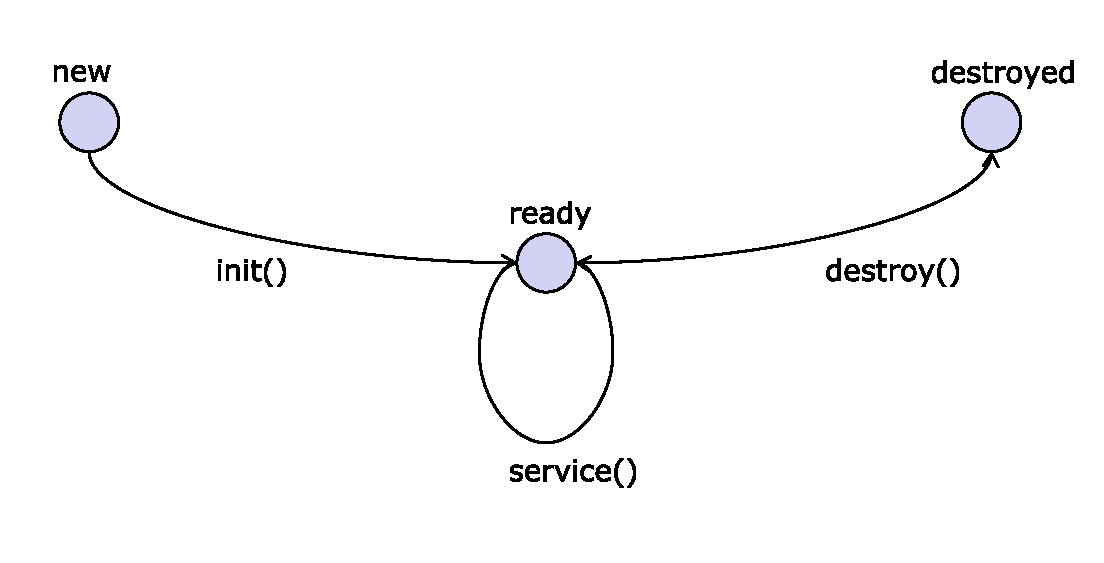
\includegraphics[width=80mm]{16/images/servlet-lifecycle}
\end{figure}

\vspace{-20px}

\paragraph{JSP (Java Server Pages)}
JSP je textový dokument obsahující statické (X)HTML tagy a JSP tagy, které umějí generovat dynamický obsah. JSP umožňuje používat kusy Java kódu v HTML stránce (scriptlet).

Za tím vším se ale skrývá servlet - \textbf{JSP jsou servlety}. JSP se při prvním použití kompiluje a vytvoří se Servlet, který dělá to, co uměla původní JSP stránka (např. do metody \texttt{doGet()} se \uv{vyprintí} celý obsah toho souboru).

\paragraph{Deskriptor} Deskriptor je konfigurační soubor s názvem \texttt{web.xml}, který musí být v každé webové aplikaci. Obsahuje mapování servletů a filtrů na requesty, kódování JSP stránek, parametry servletů a stanovuje, která stránka se zobrazí jako první (welcome-file).

\subsection{Java Bean}
Bean implementují aplikační logiku nebo vystupují v roli entit cílové domény (entita zákazník, výpůjčka...). Bean může mít lokální nebo vzdálené rozhraní podle toho, jestli se nachází na stejném stroji, nebo je na jiném stroji. Pak jsou také \textbf{EJB} (Enterprise Beans), to jsou komponenty běžící na aplikačním serveru, které jsou manažovány EJB kontejnerem. Bean je několik druhů:

\begin{itemize}[itemsep=0px]
\item \textbf{stateful} - Uchovává kontext pro každého klienta zvlášť. Je náročnější a pomalejší, proto bychom měli používat stateless, kdekoliv je to jen možné.
\item \textbf{stateless} - Jednodušší, nepamatuje si kontext volání klienta.
\item \textbf{message driven} - messaging (základní účel pro distribuované systémy).
\end{itemize}

\paragraph{Životní cyklus bean} \url{https://docs.oracle.com/javaee/6/tutorial/doc/giplj.html}

\begin{figure}[h]
\centering
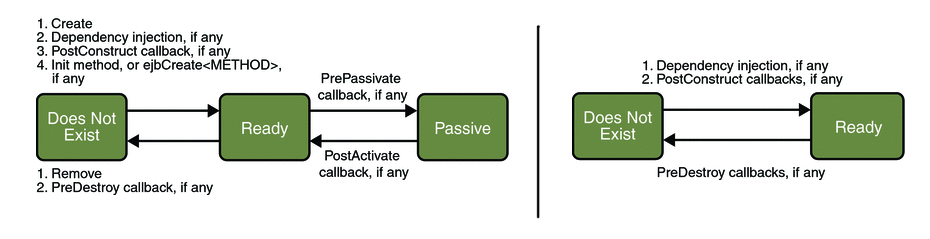
\includegraphics[width=140mm]{16/images/ejb-lifecycle}
\caption*{Životní cykly: stateful vs. stateless bean}
\end{figure}

\paragraph{Návrhové vzory využitelné v architektuře webové aplikace}
MVC, DI, Factory, Service Locator, cokoliv

\subsubsection{Inversion of Control (IoC)}
IoC, nebo také obrácené řízení, je návrhový vzor, který umožňuje \hl{uvolnit vztahy mezi jinak těsně svázanými komponentami}. DI je jedna z možností implementace IoC. V klasickém modelu programování vytváříme nějakou třídu, která pak využívá další třídy a tak dále. Tím jsou potom třídy velmi pevně svázány a změna používané třídy za jinou vyžaduje zásah do kódu. IoC umožňuje uvolnit tuto vazbu, což nejjednodušeji vystihuje Hollywoodský princip \uv{Nevolejte nám, my se ozveme.}. To je klasická odpověď, kterou dostávají amatérští herci, kteří se snaží získat v Hollywoodu nějakou roli ve filmu, seriálu apod. Proto tedy Hollywoodský princip. V podstatě to znamená, že třída nevytváří sama instance dalších tříd, které potřebuje, ale jsou jí dodány nějakým způsobem z vnějšku. Těchto způsobů existuje několik, nejznámější jsou tři:
\begin{itemize}
\item \textbf{Constructor Injection} - třídy, do nichž je vkládána instance další třídy, kterou potřebují, musejí mít vytvořen konstruktor, který umí přijímat potřebné typy objektů.
\item \textbf{Setter Injection} - třídy, do nichž jsou vkládány instance, musí mít definovány potřebné settery, setter injection používá například Spring Framework
\item \textbf{Interface Injection} - nejprve je definováno rozhraní, které určuje metody, pomocí kterých budou nastavovány instance objektů, které příslušná třída potřebuje, každá třída, která chce tyto instance využívat, musí implementovat příslušné rozhraní.
\end{itemize}
